\documentclass[10pt]{article}
\usepackage[a4paper,margin=0.72in]{geometry}
\usepackage[T1]{fontenc}
\usepackage{lmodern}
\usepackage{microtype}
\usepackage{amsmath}
\usepackage{booktabs}
\usepackage{graphicx}
\usepackage{pgfplots}
\usepackage{xcolor}
\usepackage{hyperref}
\usepackage{enumitem}
\usepackage{caption}

\definecolor{navy}{HTML}{183153}
\definecolor{linkblue}{HTML}{1F5D8C}
\hypersetup{colorlinks=true,linkcolor=navy,urlcolor=linkblue,citecolor=navy}
\setlength{\parindent}{0pt}
\setlength{\parskip}{4pt}
\setlist{nosep,leftmargin=1.4em}
\captionsetup{font=small,labelfont=bf}
\pgfplotsset{compat=1.18}

\title{\vspace{-1.1cm}\textbf{Resource-Constrained Small GPT:\\Post-Norm, RoPE, SwiGLU, and Controlled Scaling}}
\author{DASE7506 MP1 \quad Student ID: 3036779621 \quad Submission \#59}
\date{September 2026}

\begin{document}
\maketitle
\vspace{-0.7cm}

\begin{abstract}
This project improves a 1.09M-parameter classroom GPT trained from scratch on the supplied WikiText-2 data while preserving a fixed BPE-2048 tokenizer, 256-token causal evaluation windows, and strict CPU inference limits. The final model combines width scaling, SwiGLU feed-forward layers, rotary position embeddings (RoPE), eight-head attention, and block-level Post-Norm residuals. A 2,400-step schedule with validation every 300 steps selected the step-2,100 checkpoint. Validation BPB fell from 2.07109 to 1.61311, and the frozen predictor obtained 1.64120 full-test BPB. Local FP32 CPU evaluation took 15.62 seconds, used 2.29 GiB peak RSS, and required 56.13 MiB of uncompressed inference assets. Controlled comparisons show that width, RoPE, and Post-Norm gave useful gains, whereas an extra layer, a larger SwiGLU hidden dimension, grouped-query attention (GQA), and learned attention residual gates did not beat the matched full multi-head attention model. The result demonstrates that using the resource envelope effectively requires allocation and optimization choices, rather than parameter count alone.
\end{abstract}

\section{Task and evaluation protocol}

The supplied baseline is a decoder-only Transformer with four blocks, width 128, four attention heads, learned absolute position embeddings, Pre-Norm residual sublayers, and a GELU feed-forward network. It has 1,088,256 parameters and achieved 2.07109 validation BPB and 2.10127 test BPB in my local reproduction.

The target metric is bits per UTF-8 byte,
\begin{equation}
\mathrm{BPB}=\frac{-\sum_{t=1}^{N}\log p(x_t\mid x_{<t})}{\log(2)\,B},
\end{equation}
where $B$ is the raw split's UTF-8 byte count. Lower is better. The fixed evaluator scores every target once in independent causal windows of 256 tokens. Ranked evaluation must use FP32 on CPU and remain within $5\times$ baseline scoring time, 4 GiB peak RAM, and 64 MiB of uncompressed inference assets.

All development decisions and checkpoint selection used validation BPB. The test split was evaluated only after the final architecture, training recipe, and checkpoint had been frozen. All models were trained from random initialization on the supplied training text; no external data or pretrained weights were used.

\section{Final method}

\subsection{Architecture}

The final model retains four Transformer blocks but increases width to 512 and uses eight attention heads, giving a head dimension of 64. Token embeddings and the output classifier are tied. Learned absolute position embeddings are removed; RoPE rotates each query and key pair by a position-dependent angle before causal scaled dot-product attention \cite{su2021roformer}. This adds no persistent inference parameters.

The baseline GELU MLP is replaced by SwiGLU \cite{shazeer2020glu}:
\begin{equation}
\mathrm{SwiGLU}(x)=W_o\left(\mathrm{SiLU}(W_gx)\odot W_vx\right),
\end{equation}
with hidden dimension $\mathrm{round}(8d/3)=1365$ for $d=512$. This keeps the three-projection gated MLP close to the parameter cost of a conventional $4d$ two-projection MLP.

The most effective controlled architectural change was moving normalization from Pre-Norm to block-level Post-Norm while retaining the model's final LayerNorm. Each block computes
\begin{align}
h &= \mathrm{LN}\left(x+\mathrm{Attention}(x)\right),\\
y &= \mathrm{LN}\left(h+\mathrm{SwiGLU}(h)\right).
\end{align}
Post-Norm can be harder to optimize in deep Transformers \cite{xiong2020layernorm}, but this network is only four blocks deep and uses a 100-step learning-rate warm-up. Training remained finite in every logged Post-Norm run.

The frozen model has 13,659,816 parameters. Its persistent RoPE tables are registered as non-persistent buffers, so the inference bundle remains below the asset limit.

\subsection{Training and checkpoint selection}

Training uses AdamW with peak learning rate $10^{-3}$, weight decay 0.1, gradient-norm clipping at 1.0, batch size 32, sequence length 256, and seed 17. The learning rate warms up linearly for 100 steps and follows a cosine schedule with a 0.1 floor over 2,400 updates. The complete search run processes 19,660,800 targets.

Validation is evaluated every 300 steps. The best checkpoint occurred at step 2,100 after 17,203,200 targets. Validation BPB increased from 1.61311 at step 2,100 to 1.61760 at step 2,400, so retaining the best validation checkpoint avoided a small late regression.

\section{Experiments}

\subsection{Architecture path}

Table~\ref{tab:path} and Figure~\ref{fig:path} summarize the main development path. Unless noted otherwise, runs use 1,200 updates, 9,830,400 processed targets, batch size 32, and seed 17.

\begin{table}[t]
\centering
\small
\caption{Selected architecture path. Validation BPB is the development metric.}
\label{tab:path}
\begin{tabular}{lrrr}
\toprule
Model & Params (M) & Targets (M) & Val. BPB $\downarrow$\\
\midrule
Baseline & 1.088 & 9.830 & 2.07109\\
SwiGLU & 1.088 & 9.830 & 2.00788\\
SwiGLU, width 256 & 3.752 & 9.830 & 1.83197\\
SwiGLU, width 512 & 13.791 & 9.830 & 1.69071\\
+ RoPE & 13.660 & 9.830 & 1.67088\\
+ 8 heads ($d_h=64$) & 13.660 & 9.830 & 1.66762\\
+ block Post-Norm & 13.660 & 9.830 & 1.62515\\
+ 2,400-step schedule & 13.660 & 19.661 & \textbf{1.61311}\\
\bottomrule
\end{tabular}
\end{table}

\begin{figure}[t]
\centering
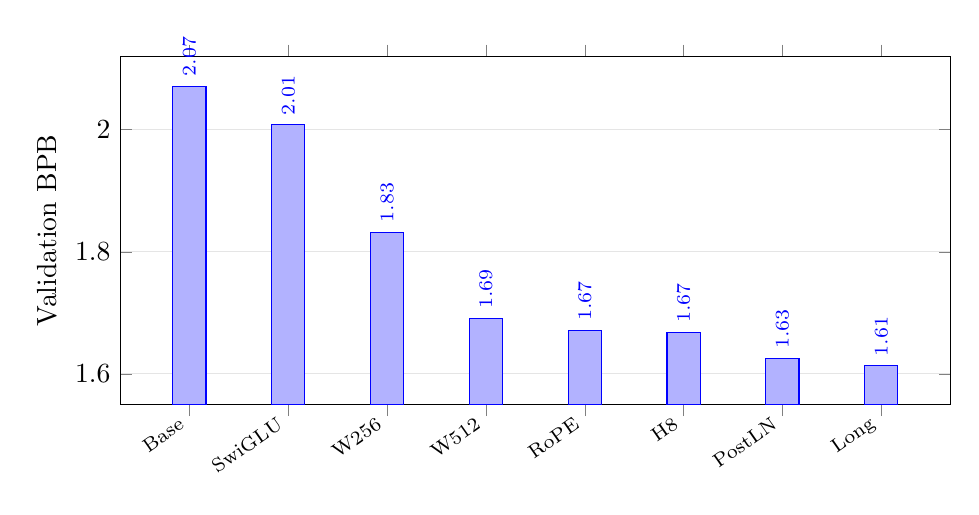
\begin{tikzpicture}
\begin{axis}[
  width=\linewidth,height=6.0cm,
  ybar,bar width=12pt,
  ymin=1.55,ymax=2.12,
  ylabel={Validation BPB},
  symbolic x coords={Base,SwiGLU,W256,W512,RoPE,H8,PostLN,Long},
  xtick=data,
  x tick label style={rotate=35,anchor=east,font=\scriptsize},
  ymajorgrids=true,grid style={gray!20},
  nodes near coords,
  nodes near coords style={font=\scriptsize,rotate=90,anchor=west},
  every axis plot/.append style={fill=linkblue,draw=linkblue}
]
\addplot coordinates {(Base,2.07109) (SwiGLU,2.00788) (W256,1.83197) (W512,1.69071) (RoPE,1.67088) (H8,1.66762) (PostLN,1.62515) (Long,1.61311)};
\end{axis}
\end{tikzpicture}
\caption{Validation BPB along the selected architecture path. The graph is descriptive rather than additive: some transitions change more than one capacity dimension. Controlled claims use the paired comparisons in the text.}
\label{fig:path}
\end{figure}

SwiGLU improved validation BPB by 0.06320 over the baseline with nearly identical parameter count. Width scaling produced the largest gains: width 256 reached 1.83197, and width 512 reached 1.69071. At width 512, replacing learned position embeddings with RoPE improved BPB by 0.01983 while slightly reducing parameters. Increasing from four to eight heads at fixed width and parameter count gave a smaller 0.00326 gain.

The cleanest ablation is Pre-Norm versus block-level Post-Norm. Both runs use width 512, eight heads, depth four, RoPE, SwiGLU, the same seed, identical parameter count, and 9.83M targets. Post-Norm reduced BPB from 1.66762 to 1.62515, a 2.55\% relative improvement. This shallow, warm-started setting therefore favored Post-Norm despite its known optimization sensitivity in deeper networks.

\subsection{Failed capacity allocations and ablations}

Table~\ref{tab:ablations} records alternatives tested after the 1,200-step Post-Norm model. Increasing depth to five blocks worsened validation BPB and produced 64.148 MiB of assets, slightly exceeding the limit. Enlarging only the SwiGLU hidden dimension added 1.84M parameters but also worsened BPB. These failures show that the final result is not explained by parameter count alone.

\begin{table}[t]
\centering
\small
\caption{Post-Norm alternatives. The matched 1,200-step control is 1.62515 BPB; the matched 2,400-step control is 1.61311 BPB.}
\label{tab:ablations}
\begin{tabular}{lrrr}
\toprule
Alternative & Params (M) & Targets (M) & Val. BPB $\downarrow$\\
\midrule
Depth 5 & 16.812 & 9.830 & 1.64338\\
GQA: width 576, Q9/KV3 & 15.367 & 9.830 & 1.62891\\
Attention residual gates & 13.660 & 9.830 & 1.62806\\
Larger SwiGLU hidden (1664) & 15.499 & 9.830 & 1.63165\\
GQA, 2,400-step schedule & 15.367 & 19.661 & 1.63180\\
Gates, 2,400-step schedule & 13.660 & 19.661 & 1.61988\\
\bottomrule
\end{tabular}
\end{table}

GQA shares key/value projections across query heads and is intended to reduce autoregressive KV-cache cost \cite{ainslie2023gqa}. The tested GQA model used width 576, nine query heads, and three KV heads. It did not beat full multi-head attention at either training budget. Moreover, the portable PyTorch CPU implementation expands K/V heads for scaled dot-product attention, so this experiment did not realize a specialized GQA-kernel speed advantage at context 256.

The gated-attention ablation added one bounded learned residual scale per block, initialized to one. After 2,400 steps, the learned scales were $[0.788,0.859,0.813,0.839]$, showing a consistent preference for smaller attention updates. Its validation BPB improved relative to the 1,200-step gated run, but remained 0.00677 above the ungated matched-schedule model. The gates learned a coherent behavior without improving the target metric.

\begin{figure}[t]
\centering
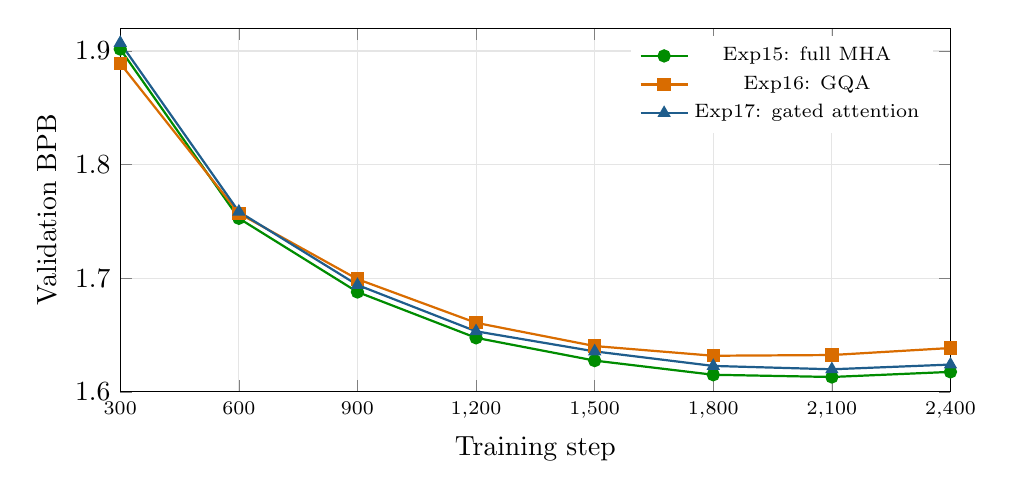
\begin{tikzpicture}
\begin{axis}[
  width=\linewidth,height=6.2cm,
  xmin=300,xmax=2400,ymin=1.60,ymax=1.92,
  xlabel={Training step},ylabel={Validation BPB},
  xtick={300,600,900,1200,1500,1800,2100,2400},
  x tick label style={font=\scriptsize},
  ymajorgrids=true,xmajorgrids=true,grid style={gray!20},
  legend style={font=\scriptsize,at={(0.98,0.98)},anchor=north east,draw=none,fill=white},
  mark size=2pt
]
\addplot[color=green!55!black,thick,mark=*] coordinates {(300,1.90162) (600,1.75273) (900,1.68789) (1200,1.64756) (1500,1.62753) (1800,1.61506) (2100,1.61311) (2400,1.61760)};
\addlegendentry{Exp15: full MHA}
\addplot[color=orange!85!black,thick,mark=square*] coordinates {(300,1.88898) (600,1.75709) (900,1.69921) (1200,1.66078) (1500,1.64033) (1800,1.63180) (2100,1.63243) (2400,1.63861)};
\addlegendentry{Exp16: GQA}
\addplot[color=linkblue,thick,mark=triangle*] coordinates {(300,1.90708) (600,1.75857) (900,1.69407) (1200,1.65330) (1500,1.63563) (1800,1.62284) (2100,1.61988) (2400,1.62404)};
\addlegendentry{Exp17: gated attention}
\end{axis}
\end{tikzpicture}
\caption{Validation curves for matched 2,400-step schedules. Full multi-head attention remains best. All three curves turn upward after their selected checkpoint, supporting validation-based checkpoint selection.}
\label{fig:curves}
\end{figure}

\section{Frozen test result and resource compliance}

After Exp15 was selected using validation, its step-2,100 checkpoint was frozen and evaluated on the complete test split. Table~\ref{tab:final} reports the final result and local resource measurements. A second evaluation reproduced the BPB exactly.

\begin{table}[t]
\centering
\small
\caption{Frozen final predictor. Timing is local and machine-dependent.}
\label{tab:final}
\begin{tabular}{lrr}
\toprule
Metric & Measured & Limit / reference\\
\midrule
Validation BPB & 1.61311 & development only\\
Full-test FP32 BPB & \textbf{1.64120} & baseline 2.10127\\
Test scoring time & 15.615 s & $3.74\times$ local baseline\\
Peak test RSS & 2.287 GiB & 4 GiB\\
Inference assets & 56.128 MiB & 64 MiB\\
Parameters & 13.660 M & constrained indirectly\\
\bottomrule
\end{tabular}
\end{table}

The final test BPB improves over the reproduced baseline by 0.46006, or 21.9\% relative. Evaluation cost rises because width increases from 128 to 512, but the local time ratio remains below $5\times$. The checkpoint, implementation, and configuration leave 7.87 MiB of asset headroom, while peak RSS leaves 1.71 GiB of memory headroom.

\section{Critical analysis and limitations}

The evidence supports three practical conclusions. First, capacity helped most when allocated to model width; extra depth and a larger feed-forward hidden dimension did not improve generalization under the same target budget. Second, low-overhead structural choices---RoPE and Post-Norm in particular---improved BPB without increasing inference assets. Third, longer training gave a smaller gain than the main architecture changes and required validation checkpointing to avoid late degradation.

Several limitations constrain interpretation:
\begin{itemize}
\item Most comparisons use one seed. Small differences, especially the four-versus-eight-head gain, may be within seed variance.
\item Repeated architectural search reuses one validation set. Although the test split was reserved for the frozen method, extensive validation reuse can still overfit model-development decisions.
\item The 300-step checkpoint interval is coarse; the true optimum may lie between recorded checkpoints.
\item Resource measurements were made on one macOS CPU. BPB reproduced exactly, but scoring time and RSS will vary across systems.
\item Conclusions are specific to WikiText-2, BPE-2048, context 256, and this small-model regime. GQA may be more useful with long-context decoding and specialized kernels.
\end{itemize}

Future work should prioritize multi-seed confirmation of Post-Norm, narrower schedule searches fixed in advance, and parameter reallocations that preserve a larger asset margin. It should not use the test set for selection.

\section{Reproducibility and assistance disclosure}

The repository contains the fixed evaluator, supplied data and tokenizer, final source, exact training command, frozen result JSON, experiment log, and ablation snapshots. The checkpoint is distributed separately with its SHA-256 hash. All architectural hypotheses, experiment directions, comparison choices, and final model-selection decisions were proposed and made by the student. OpenAI ChatGPT/Codex was used as a technical assistant to explain the starter code, help translate the student's proposed experiments into code and reproducible commands, review implementation details, organize recorded measurements, and assist with editing this report. The student launched all training runs, inspected the outputs, interpreted the experimental results, and reviewed the final implementation and analysis. No AI-generated or external text was used as training data.

\begin{thebibliography}{9}
\bibitem{vaswani2017attention}
A. Vaswani et al. ``Attention Is All You Need.'' \emph{NeurIPS}, 2017.

\bibitem{shazeer2020glu}
N. Shazeer. ``GLU Variants Improve Transformer.'' arXiv:2002.05202, 2020. \url{https://arxiv.org/abs/2002.05202}

\bibitem{su2021roformer}
J. Su, Y. Lu, S. Pan, A. Murtadha, B. Wen, and Y. Liu. ``RoFormer: Enhanced Transformer with Rotary Position Embedding.'' arXiv:2104.09864, 2021. \url{https://arxiv.org/abs/2104.09864}

\bibitem{xiong2020layernorm}
R. Xiong et al. ``On Layer Normalization in the Transformer Architecture.'' \emph{ICML}, 2020. \url{https://proceedings.mlr.press/v119/xiong20b.html}

\bibitem{ainslie2023gqa}
J. Ainslie et al. ``GQA: Training Generalized Multi-Query Transformer Models from Multi-Head Checkpoints.'' arXiv:2305.13245, 2023. \url{https://arxiv.org/abs/2305.13245}

\bibitem{merity2017pointer}
S. Merity, C. Xiong, J. Bradbury, and R. Socher. ``Pointer Sentinel Mixture Models.'' \emph{ICLR}, 2017. \url{https://arxiv.org/abs/1609.07843}
\end{thebibliography}

\end{document}
